\documentclass[letterpaper, 12pt]{article}

% \usepackage[showframe, margin=1in, top=0.25in, bottom=0.25in, includeheadfoot, headheight=0.5in]{geometry}
\usepackage[margin=1in, top=0.25in, bottom=0.25in, includeheadfoot, headheight=0.5in]{geometry}

\AddToHook{cmd/section/before}{\clearpage}

\usepackage[table]{xcolor}
\colorlet{listingback}{gray!20}
\definecolor{headingcolor}{RGB}{110,34,54}

\usepackage{fancyhdr}
\renewcommand{\sectionmark}[1]{\markboth{#1}{#1}}

% Used to detect whether a section is an appendix to print the right thing in the footer
\usepackage{etoolbox}
\newtoggle{inappendix}
\pretocmd{\appendix}{\clearpage\toggletrue{inappendix}}{}{}

% Save standard definitions for head and foot rules (lines separating header and footer from text)
\let\HeadRule\headrule
\let\FootRule\footrule
% Add color to the standard definitions
\renewcommand{\headrule}{\color{headingcolor}\HeadRule}
\renewcommand{\footrule}{\textcolor{headingcolor}{\FootRule}}

% IMPORTANT: This command should not be called directly. Use \preamble.
% Macro to insert the title page for each lab.
% The argument is the title of the lab.
\newcommand{\inserttitlepage}[1]
{
    \begin{titlepage}
    \centering
    
\includegraphics[scale=0.5]{images/nexus_lab_logo.png}

    \vspace*{\baselineskip}

    \textbf{\Large OpenStack Labs}

    \vspace*{\baselineskip}

    \textbf{\Large #1}
    \vspace*{\fill}
\end{titlepage}
}

% IMPORTANT: This command should not be called directly. Use \preamble.
% Macro to define header and footer for each lab.
% The argument is the title of the lab.
\newcommand{\headfoot}[1]
{
    \fancypagestyle{fancy}
    {
        \fancyhf{}
        \fancyhead[L]{\footnotesize #1}
        \fancyhead[R]{
\includegraphics[height=0.85\headheight]{images/nexus_lab_logo.png}}
        \fancyfoot[L]{%
            \footnotesize%
            \ifnum\value{section}>0%
            \iftoggle{inappendix}{Appendix \thesection: \rightmark}{Section \thesection: \rightmark}%
            \fi}
        \fancyfoot[R]{\footnotesize\thepage}
        \renewcommand{\headrulewidth}{1.5pt}
        \renewcommand{\footrulewidth}{1.5pt}
    }
}

% Macro to insert title page, define header and footer, and insert table of contents and about section for each lab.
% The argument is the title of the lab.
\newcommand{\preamble}[1]
{
    \pagenumbering{roman}
    \inserttitlepage{#1}
    \headfoot{#1}

    % Insert table of contents
    \pagestyle{fancy}
    \tableofcontents
    \clearpage

    \section*{About This Document}
    \label{sec:about_this_document}
    \begin{itemize}
        \item This document was developed by a team at the University of Tennessee at Chattanooga led by Dr. Mengjun Xie
        (\href{mailto:mengjun-xie@utc.edu}{\textbf{mengjun-xie@utc.edu}}).
        \item The development of this document was supported by a National Centers of Academic Excellence in Cybersecurity Grant (\#H98230-20-1-0351), housed at the National Security Agency.
        \item This document is licensed with a Creative Commons Attribution 4.0 International License.
    \end{itemize}
    \clearpage
}

% Macro to insert the Lab Settings page for each lab. Call after the Introduction and Objectives sections.
\newcommand{\labsettings}
{
    \section*{Lab Settings}
    \label{sec:lab_settings}
    \addcontentsline{toc}{section}{\nameref{sec:lab_settings}}
    The information in the table below will be needed in order to complete the lab.
    The task sections below provide details on the use of this information.
    \begin{table*}[htbp]
        \centering
        \begin{tabular}{|c|c|c|c|}
            \hline
            \rowcolor{gray!20} \textbf{Virtual Machine} & \textbf{IP Address} & \textbf{Account} & \textbf{Password} \\
            \hline
            \multirow{2}{*}{\texttt{workstation}} & \multirow[t]{2}{*}{\texttt{ens3: 192.168.1.21}}  & \multirow{2}{*}{\texttt{ubuntu}} & \multirow{2}{*}{\texttt{ubuntu}} \\
                                                  & \multirow[t]{2}{*}{\texttt{ens4: 172.25.250.21}} &                                  &                                  \\
            \hline
            \multirow{2}{*}{\texttt{devstack}}    & \multirow[t]{2}{*}{\texttt{ens3: 192.168.20}}    & \multirow{2}{*}{\texttt{ubuntu}} & \multirow{2}{*}{\texttt{ubuntu}} \\
                                                  & \multirow[t]{2}{*}{\texttt{ens4: 172.25.250.20}} &                                  &                                  \\
            \hline
        \end{tabular}
    \end{table*}
    \clearpage

    % IMPORTANT(lucas): If another frontmatter section ever gets placed after this, this command needs to be moved
    % to the end of that section.
    % I have placed this here and not in each lab purely for convenience and to ensure I don't forget any.
    \pagenumbering{arabic}
}

% Sans-serif font
\renewcommand{\familydefault}{\sfdefault}
\newcommand{\texttildemid}{{\raisebox{0.5ex}{\texttildelow}}}

\usepackage{enumitem}
\renewcommand{\labelenumi}{\textbf{\thesection.\arabic{enumi}.}}

% Try to forbid widows and orphans
\widowpenalty10000
\clubpenalty10000

\usepackage{graphicx}
\usepackage{hyperref}
\hypersetup{colorlinks=true,linkcolor=black,urlcolor={[named] headingcolor}}

\usepackage{sectsty}
\sectionfont{\color{headingcolor}}

% Table of Contents
\usepackage{bookmark}
\usepackage[titles]{tocloft}
\usepackage[title]{appendix}
\renewcommand{\cfttoctitlefont}{\Large\bfseries\color{headingcolor}}
\renewcommand{\cftsecfont}{\normalfont\normalsize}
\renewcommand{\cftsecpagefont}{\normalfont\normalsize}
\renewcommand{\cftdotsep}{0} % Make dots small and close together
\renewcommand{\cftsecleader}{\cftdotfill{\cftdotsep}} % Add dots after section titles
% Make dots go all the way to the page number
\renewcommand{\cftsecfillnum}[1]{{\cftsecleader}\nobreak{\cftsecpagefont #1}\cftsecafterpnum\par}

\usepackage{multirow}
\setlength{\tabcolsep}{16pt}
\renewcommand{\arraystretch}{1.1}

% For nice-looking boxes
\usepackage[most]{tcolorbox}
\usepackage{listings}
\usepackage{lstautogobble}
\lstset{
  frame=none,
  language=Bash,
  showstringspaces=false,
  basicstyle={\linespread{1.1}\footnotesize\ttfamily\selectfont},
  numbers=none,
  breaklines=true,
  breakatwhitespace=true,
  tabsize=3,
  columns=fullflexible,
  keepspaces=true,
  escapeinside={(*@}{@*)},
  literate={~}{{\texttildemid}}{1}
           {\#}{\#}{1},
  autogobble=true
}

\tcolorboxenvironment{lstlisting}
{
    spartan,
    colframe=gray!50,
    boxsep=0mm,
    left=1mm,
    right=1mm,
    top=-1mm,
    bottom=-1mm,
    colback=gray!20
}

% Hacky solution for now, would like to have just one environment and make several tcolorboxes by passing different
% colors as parameters, but that is giving errors
\makeatletter
\tcbset{
  note/.style={%
        enhanced,
        breakable,
        colback=blue!10!white,
        colframe=blue!80!white,
        attach boxed title to top left={yshift*=-\tcboxedtitleheight},
        title={#1},
        boxed title size=title,
        boxed title style={%
            sharp corners,
            rounded corners=northwest,
            colback=tcbcolframe,
            boxrule=0pt,
        },
        underlay boxed title={%
            \path[fill=tcbcolframe] (title.south west)--(title.south east)
                to[out=0, in=180] ([xshift=5mm]title.east)--
                (title.center-|frame.east)
                [rounded corners=\kvtcb@arc] |-
                (frame.north) -| cycle;
        },
    }
}
\makeatother

\makeatletter
\tcbset{
    stop/.style={%
        enhanced,
        breakable,
        colback=white,
        colback=red!10!white,
        colframe=red!80!white,
        attach boxed title to top left={yshift*=-\tcboxedtitleheight},
        title={#1},
        boxed title size=title,
        boxed title style={%
            sharp corners,
            rounded corners=northwest,
            colback=tcbcolframe,
            boxrule=0pt,
        },
        underlay boxed title={%
            \path[fill=tcbcolframe] (title.south west)--(title.south east)
                to[out=0, in=180] ([xshift=5mm]title.east)--
                (title.center-|frame.east)
                [rounded corners=\kvtcb@arc] |-
                (frame.north) -| cycle;
        },
    }
}
\makeatother

\makeatletter
\tcbset{
    tip/.style={%
        enhanced,
        breakable,
        colback=white,
        colback=green!10,
        colframe=green!70!black,
        attach boxed title to top left={yshift*=-\tcboxedtitleheight},
        fonttitle=\bfseries,
        title={#1},
        boxed title size=title,
        boxed title style={%
            sharp corners,
            rounded corners=northwest,
            colback=tcbcolframe,
            boxrule=0pt,
        },
        underlay boxed title={%
            \path[fill=tcbcolframe] (title.south west)--(title.south east)
                to[out=0, in=180] ([xshift=5mm]title.east)--
                (title.center-|frame.east)
                [rounded corners=\kvtcb@arc] |-
                (frame.north) -| cycle;
        },
    }
}
\makeatother

% The commands below define environments for colored boxes. They are used like
% \begin{notebox}
% ...
% \end{notebox}
\newtcolorbox{notebox}{note={Note}}
\newtcolorbox{stopbox}{stop={Stop}}
\newtcolorbox{tipbox}{tip={Tip}}


\begin{document}
\begin{titlepage}
    \centering
    
\includegraphics[scale=0.5]{images/nexus_lab_logo.png}

    \vspace*{\baselineskip}

    \textbf{\Large OpenStack Labs}

    \vspace*{\baselineskip}

    \textbf{\Large Lab 09: Customizing Instances}
    \vspace*{\fill}
\end{titlepage}

\fancypagestyle{fancy}
{
    \fancyhf{}
    \fancyhead[L]{\footnotesize Lab 09: Customizing Instances}
    \fancyhead[R]{
\includegraphics[height=0.85\headheight]{images/nexus_lab_logo.png}}
    \fancyfoot[R]{\footnotesize\thepage}
    \renewcommand{\headrulewidth}{0pt}
}

\pagestyle{fancy}
\tableofcontents
\clearpage

\section*{Introduction}
\label{sec:introduction}
\addcontentsline{toc}{section}{\nameref{sec:introduction}}
In this lab, you will use the \textbf{\texttt{cloud-init}} utility to customize OpenStack instances.

\section*{Objectives}
\label{sec:objectives}
\addcontentsline{toc}{section}{\nameref{sec:objectives}}
\begin{itemize}[itemsep=0pt]
    \item Customize an instance with \textbf{\texttt{cloud-init}}.
    \item Verify instance customization.
\end{itemize}
\clearpage

\section*{Lab Settings}
\label{sec:lab_settings}
\addcontentsline{toc}{section}{\nameref{sec:lab_settings}}
The information in the table below will be needed in order to complete the lab. The task sections below provide details
on the use of this information.
\begin{table*}[htbp]
\centering
\begin{tabular}{|c|c|c|c|}
    \hline
    \rowcolor{gray!20} \textbf{Virtual Machine} & \textbf{IP Address} & \textbf{Account} & \textbf{Password} \\
    \hline
    \multirow{2}{*}{\texttt{workstation}} & \multirow[t]{2}{*}{\texttt{ens3: 192.168.1.21}}  & \multirow{2}{*}{\texttt{ubuntu}} & \multirow{2}{*}{\texttt{ubuntu}} \\
                                          & \multirow[t]{2}{*}{\texttt{ens4: 172.25.250.21}} &                                  &                                  \\
    \hline
    \multirow{2}{*}{\texttt{devstack}}    & \multirow[t]{2}{*}{\texttt{ens3: 192.168.1.20}}  & \multirow{2}{*}{\texttt{ubuntu}} & \multirow{2}{*}{\texttt{ubuntu}} \\
                                          & \multirow[t]{2}{*}{\texttt{ens4: 172.25.250.20}} &                                  &                                  \\
    \hline
\end{tabular}
\end{table*}
\clearpage

\section{Creating Customized Instances}
\label{sec:creating_customized_instances}
In this task, you will customize two instances using \textbf{\texttt{cloud-init}} capabilities and features. You will
log into the first instance to confirm \textbf{\texttt{cloud-init}} is up and running.

\begin{enumerate}
    % TODO(lucas): Viewing the default Apache web page will require being able to access the instance
    % from the workstation, which is currently not working
    \item Open the web browser and navigate to \textbf{192.168.1.20}. Log into the dashboard as \textbf{admin} with the
    password \textbf{secret}.

    \item Switch to the \textbf{demo} project. Navigate to \textbf{Admin $>$ Network $>$ Routers}. Check the box in the
    same row as \textbf{router1}, then click \textbf{Delete Routers}.

    \begin{center}
        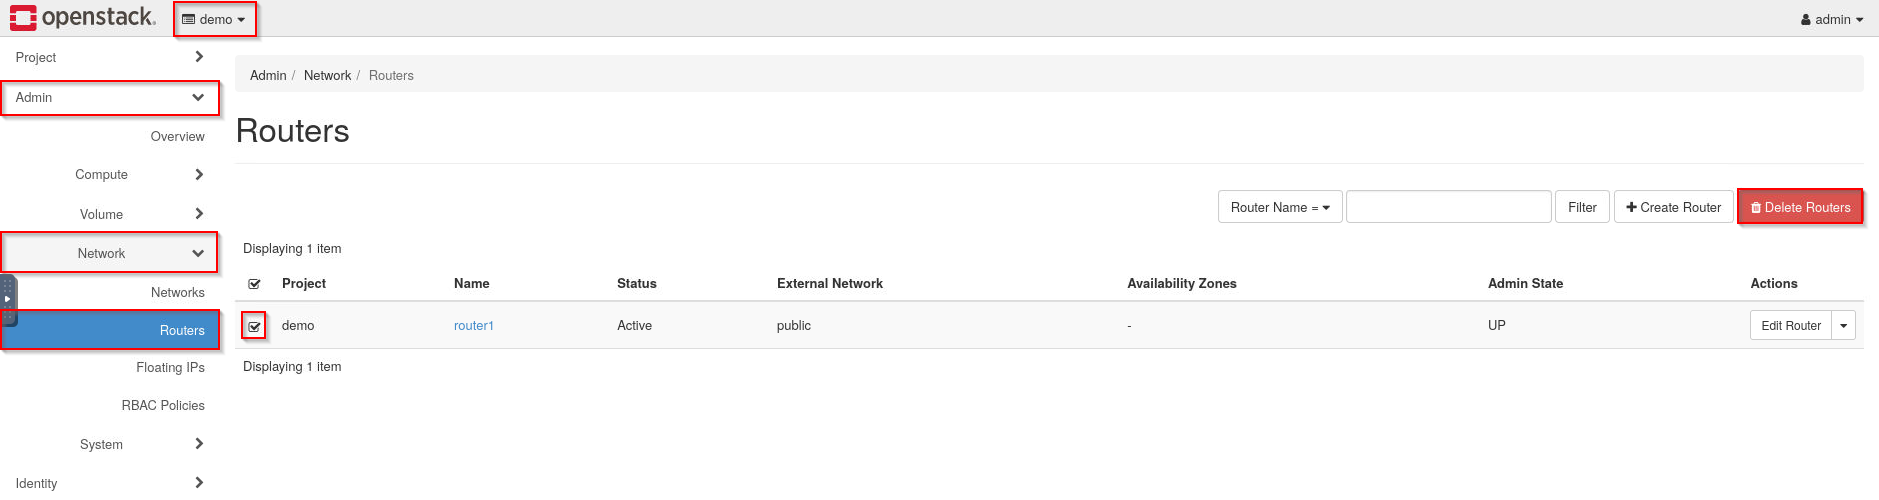
\includegraphics[width=\linewidth]{images/part1/step2.png}
    \end{center}

    \item In the \textit{Confirm Delete Routers} dialog box that pops up, click \textbf{Delete Routers}.

    \begin{center}
        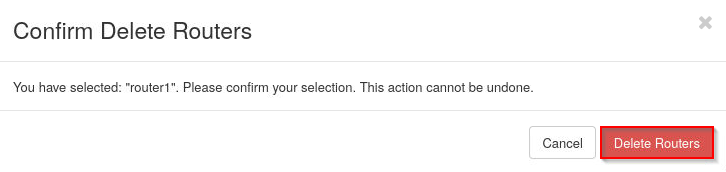
\includegraphics[width=\linewidth]{images/part1/step3.png}
    \end{center}

    \item Now, navigate to \textbf{Networks}. Check the box in the same row as \textbf{public}, then click
    \textbf{Delete Networks}.

    \begin{center}
        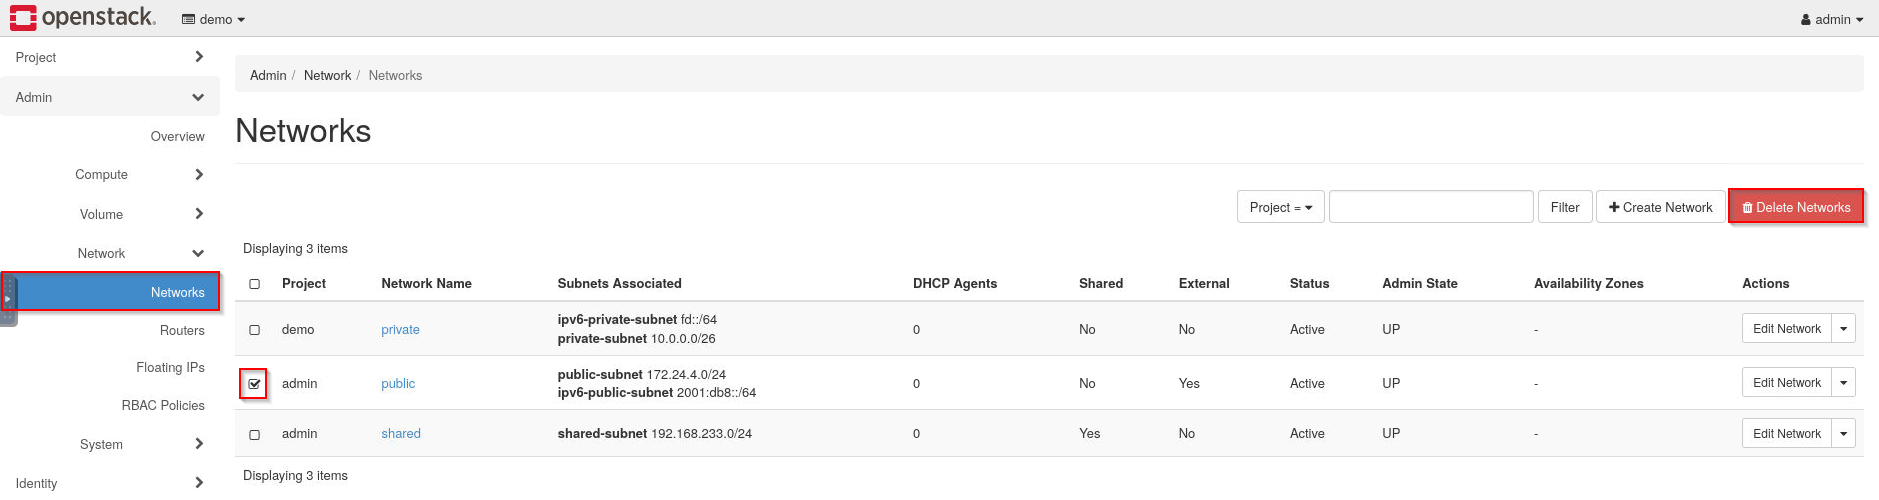
\includegraphics[width=\linewidth]{images/part1/step4.png}
    \end{center}

    \item In the \textit{Confirm Delete Networks} dialog box that pops up, click \textbf{Delete Networks}.

    \begin{center}
        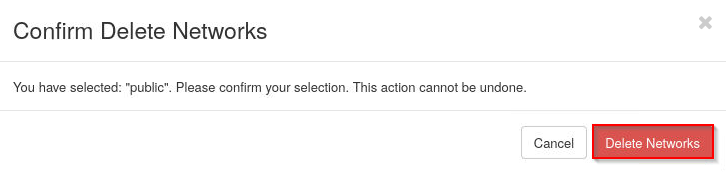
\includegraphics[width=\linewidth]{images/part1/step5.png}
    \end{center}

    \item Leave the web browser open and open a terminal window. Source the keystone credentials for the \textbf{admin}
    user.
\begin{lstlisting}
ubuntu@workstation:~$ source ~/keystonerc-admin
\end{lstlisting}

    \begin{center}
        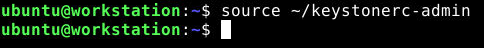
\includegraphics[width=\linewidth]{images/part1/step6.png}
    \end{center}

    \item A few resources need to be created to help with customizing the instances. First, create an external network
    named \textbf{external}. Set the network type to \textbf{flat} and the physical network to \textbf{public}. Set the
    network as shared and external.
\begin{lstlisting}
ubuntu@workstation:~$ openstack network create external \
> --external --share \
> --provider-network-type flat \
> --provider-physical-network public
\end{lstlisting}

    \begin{center}
        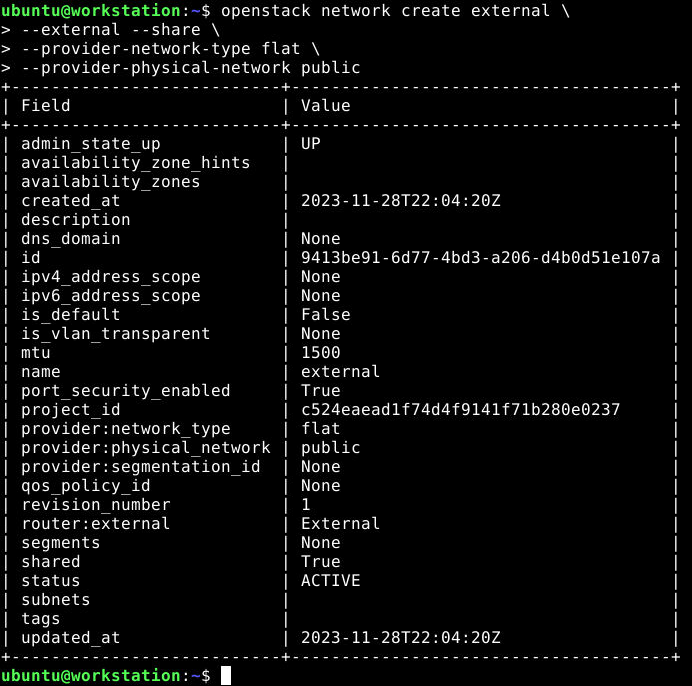
\includegraphics[width=\linewidth]{images/part1/step7.png}
    \end{center}

    \begin{tipbox}{}
        WHen typing the command, make sure there is a space between \texttt{external} and the \texttt{\textbackslash}
        character, and press \textbf{Enter} to get the \texttt{>} and continue typing the rest of the command.
    \end{tipbox}

    \item Create a subnet named \textbf{subext} in the \textbf{external} network. Give the subnet a range of
    \textbf{172.25.250.60} to \textbf{172.25.250.80}. Disable DHCP services for the subnet and use the address
    \textbf{172.25.250.254} as the gateway as well as the DNS name server.
\begin{lstlisting}
ubuntu@workstation:~$ openstack subnet create \
> --subnet-range 172.25.250.0/24 \
> --no-dhcp \
> --gateway 172.25.250.254 \
> --dns-nameserver 172.25.250.254 \
> --allocation-pool start=172.25.250.60,end=172.25.250.80 \
> --network external \
> subext
\end{lstlisting}

    \begin{center}
        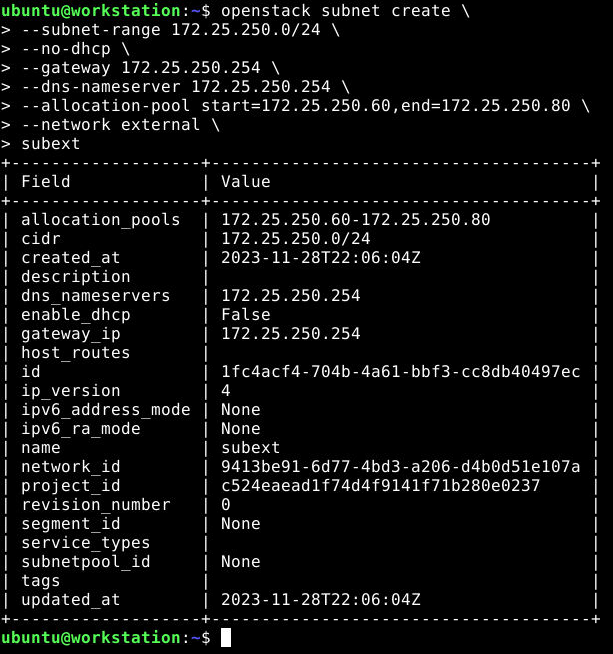
\includegraphics[width=\linewidth]{images/part1/step8.png}
    \end{center}

    \item From the floating IP pool in the \textbf{external} network, create a floating IP.
\begin{lstlisting}
ubuntu@workstation:~$ openstack floating ip create external
\end{lstlisting}

    \begin{center}
        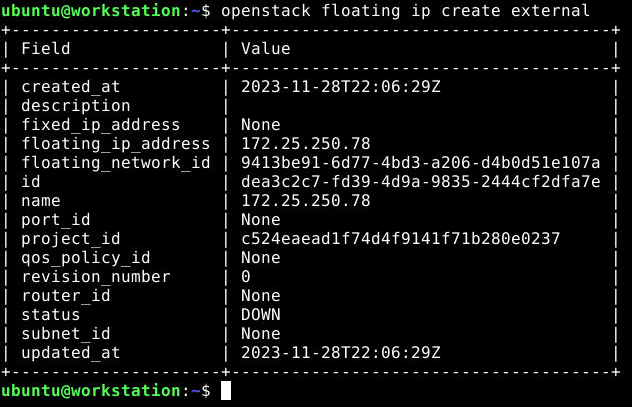
\includegraphics[width=\linewidth]{images/part1/step9.png}
    \end{center}

\item Create a router named \textbf{exercise-router}.
\begin{lstlisting}
ubuntu@workstation:~$ openstack router create exercise-router
\end{lstlisting}

    \begin{center}
        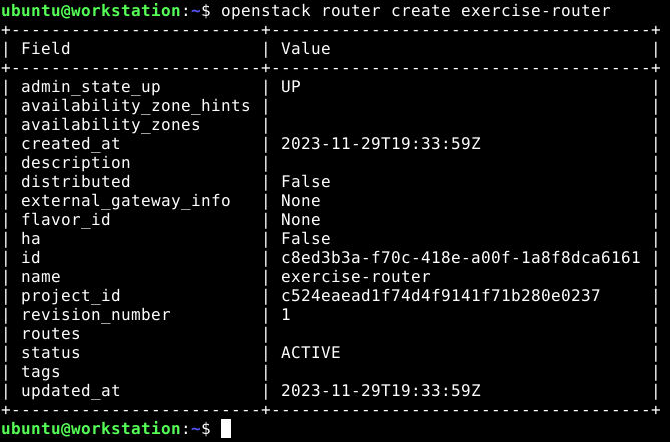
\includegraphics[width=\linewidth]{images/part1/step10.png}
    \end{center}

    \item Connect the router to the \textbf{shared-subnet} subnet.
\begin{lstlisting}
ubuntu@workstation:~$ openstack router add subnet \
> exercise-router shared-subnet
\end{lstlisting}

    \begin{center}
        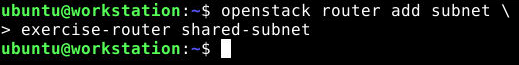
\includegraphics[width=\linewidth]{images/part1/step11.png}
    \end{center}

    \item Set the \textbf{external} network as the gateway for the router.
\begin{lstlisting}
ubuntu@workstation:~$ openstack router set \
> --external-gateway external \
> exercise-router
\end{lstlisting}

    \begin{center}
        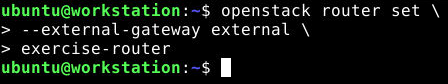
\includegraphics[width=\linewidth]{images/part1/step12.png}
    \end{center}

    \item Create the key pair \textbf{dev-keypair} and save the private key to the file
\textbf{\texttildemid/Downloads/dev-keypair.pem}.
\begin{lstlisting}
ubuntu@workstation:~$ openstack keypair create \
> dev-keypair > ~/Downloads/dev-keypair.pem
\end{lstlisting}

    \begin{center}
        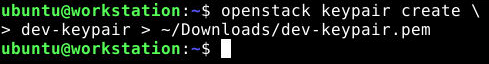
\includegraphics[width=\linewidth]{images/part1/step13.png}
    \end{center}

    \item the \textbf{\texttt{chmod}} command with a mode of \textbf{600} to make it so that the \textbf{ubuntu} user
has read/write permissions on the file, and groups and other users have no permissions to the file.
\begin{lstlisting}
ubuntu@workstation:~$ chmod 600 ~/Downloads/dev-keypair.pem
\end{lstlisting}

    \begin{center}
        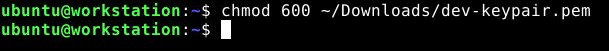
\includegraphics[width=\linewidth]{images/part1/step14.png}
    \end{center}

    \item Create the \textbf{dev-secgroup} security group.
\begin{lstlisting}
ubuntu@workstation:~$ openstack security group \
> create dev-secgroup
\end{lstlisting}

    \begin{center}
        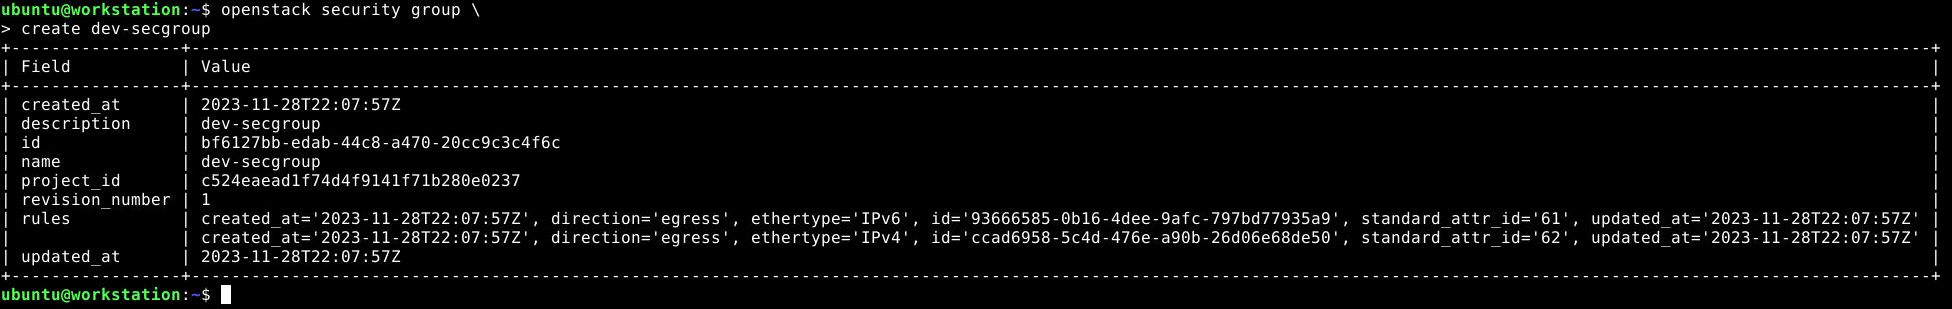
\includegraphics[width=\linewidth]{images/part1/step15.png}
    \end{center}

    \item Add a security rule in the \textbf{dev-secgroup} security group to allow remote ICMP traffic.
\begin{lstlisting}
ubuntu@workstation: openstack security group \
> rule create \
> --protocol icmp \
> dev-secgroup
\end{lstlisting}

    \begin{center}
        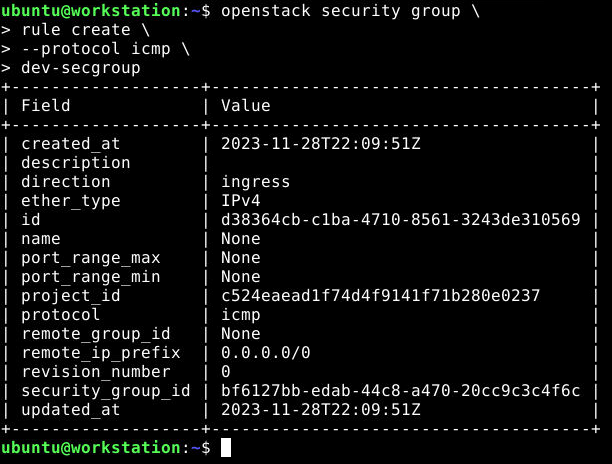
\includegraphics[width=\linewidth]{images/part1/step16.png}
    \end{center}

    \item Add another security rule to allow remote connection using SSH on the default port 22.
\begin{lstlisting}
ubuntu@workstation:~$ openstack security group \
> rule create \
> --protocol tcp \
> --dst-port 22 \
> dev-secgroup
\end{lstlisting}

    \begin{center}
        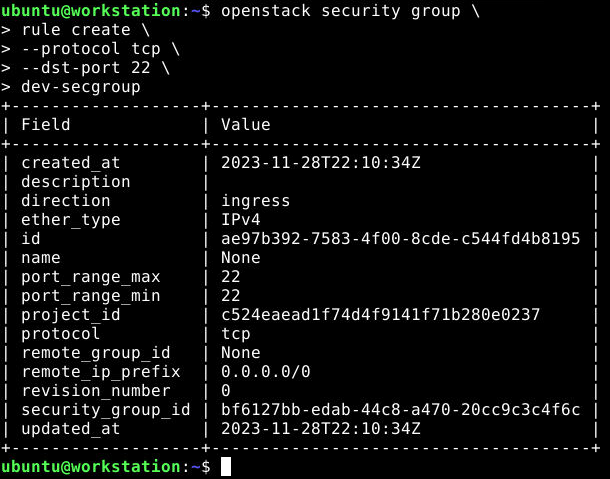
\includegraphics[width=\linewidth]{images/part1/step17.png}
    \end{center}

    \item Now that the necessary resources have been created, focus back to the web browser. Navigate to
    \textbf{Project $>$ Compute $>$ Instances}, then click \textbf{Launch Instance}.

    \begin{center}
        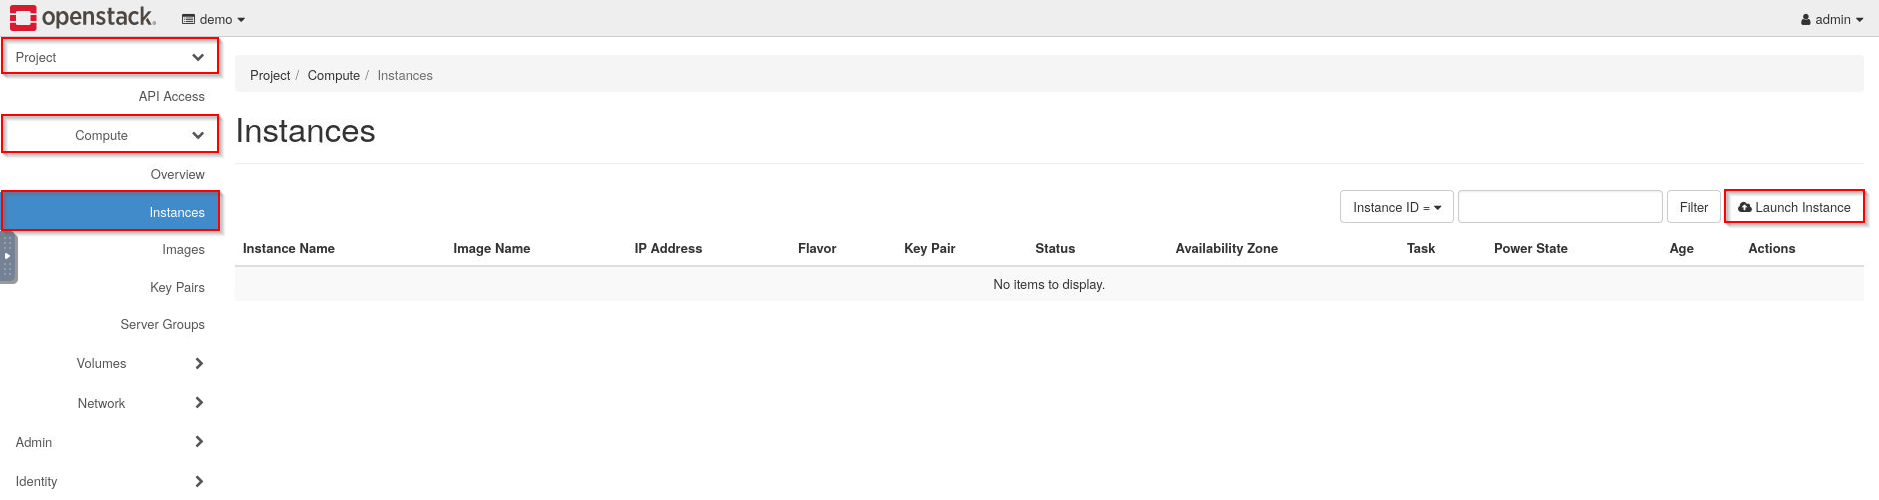
\includegraphics[width=\linewidth]{images/part1/step18.png}
    \end{center}

    \item In the \textit{Details} tab, enter \textbf{instance1} in the \textit{Instance Name} field and click
    \textbf{Next}.

    \begin{center}
        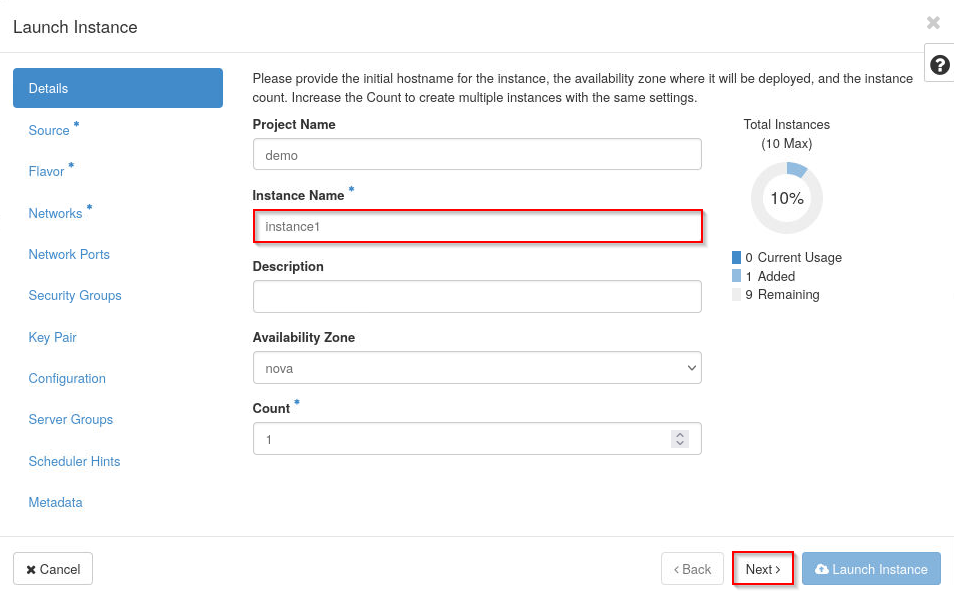
\includegraphics[width=\linewidth]{images/part1/step19.png}
    \end{center}

    \item In the \textit{Source} tab, make sure \textbf{Image} is selected in the \textit{Select Boot Source} dropdown
    and click \textbf{No} under \textit{Create New Volume}. Select the \textbf{ubuntu} image by clicking the $\uparrow$
    symbol in the same row. Click \textbf{Next}.

    \begin{center}
        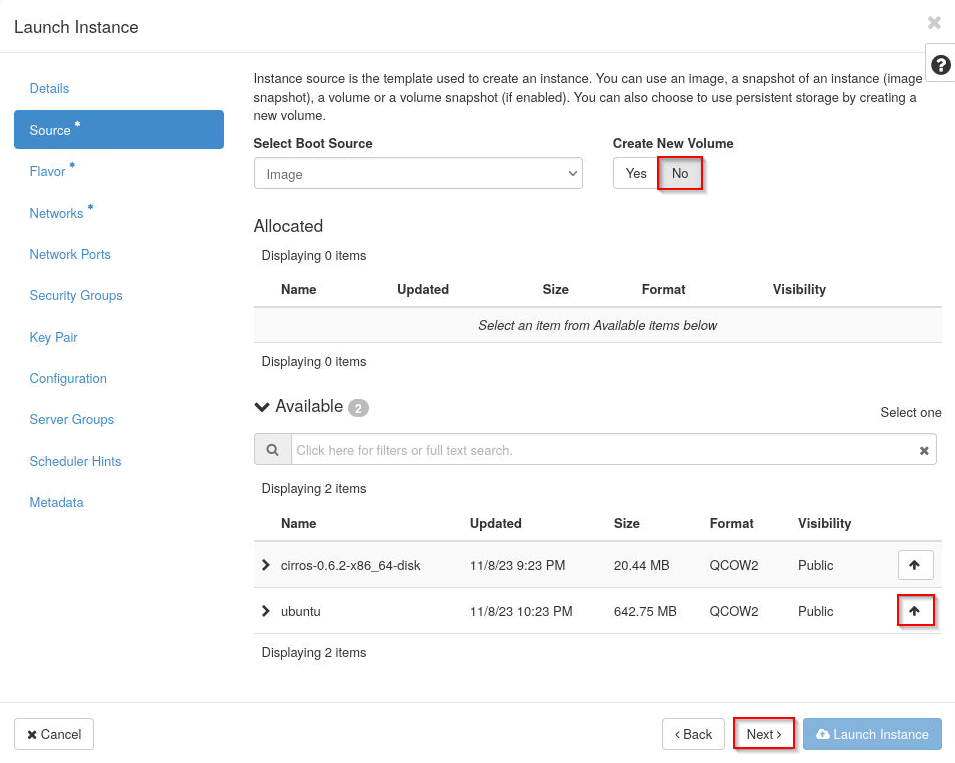
\includegraphics[width=\linewidth]{images/part1/step20.png}
    \end{center}

    \begin{stopbox}{}
        Before proceeding to the next step, confirm that \textbf{ubuntu} appears underneath the \textit{Allocated}
        section.
    \end{stopbox}

    \item In the \textit{Flavor} tab, click the $\uparrow$ symbol in the same row as \textbf{m1.small}. Click \textbf{Next}.

    \begin{center}
        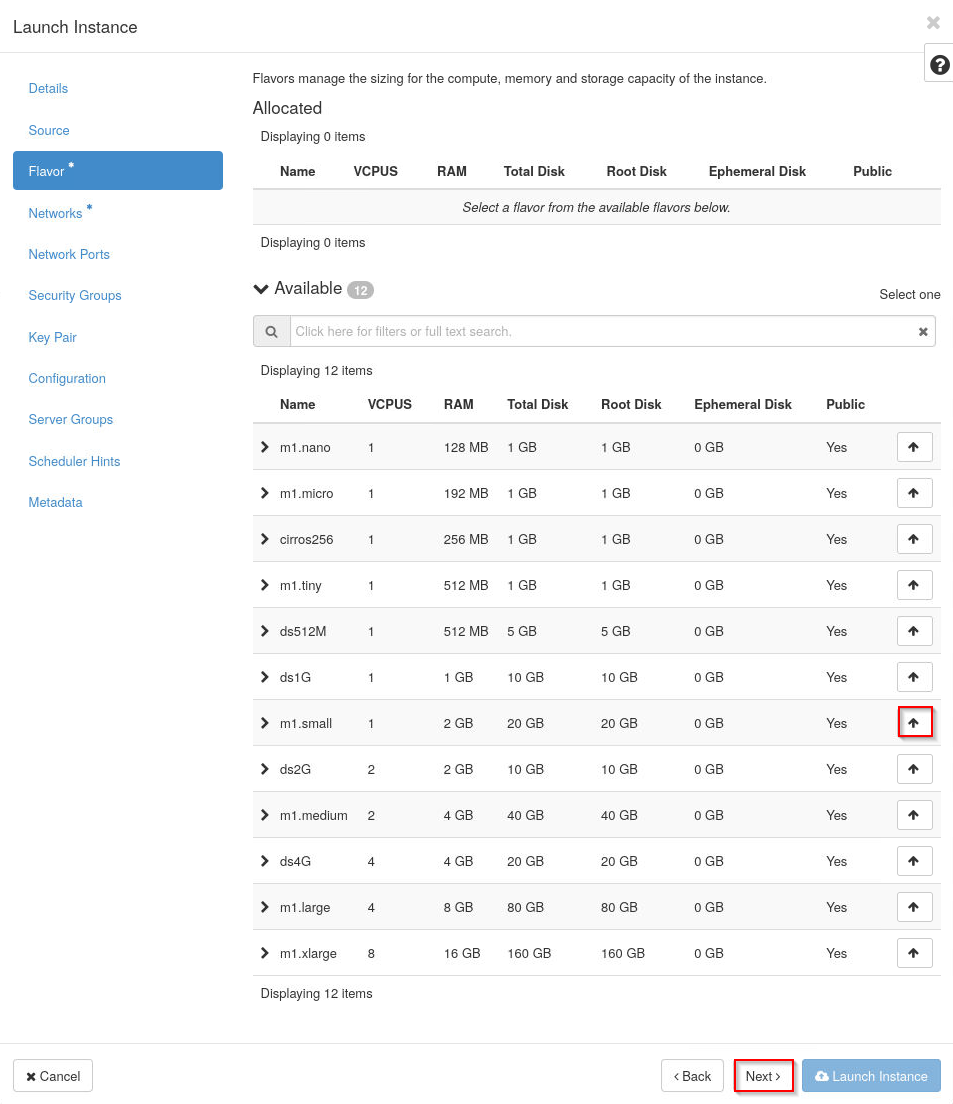
\includegraphics[width=\linewidth]{images/part1/step21.png}
    \end{center}

    \begin{stopbox}{}
        Before proceeding to the next step, confirm that \textbf{m1.small} appears underneath the \textit{Allocated}
        section.
    \end{stopbox}

    \item In the \textit{Networks} tab, click the $\uparrow$ symbol in the same row as \textbf{shared}. Click
    \textbf{Next}.

    \begin{center}
        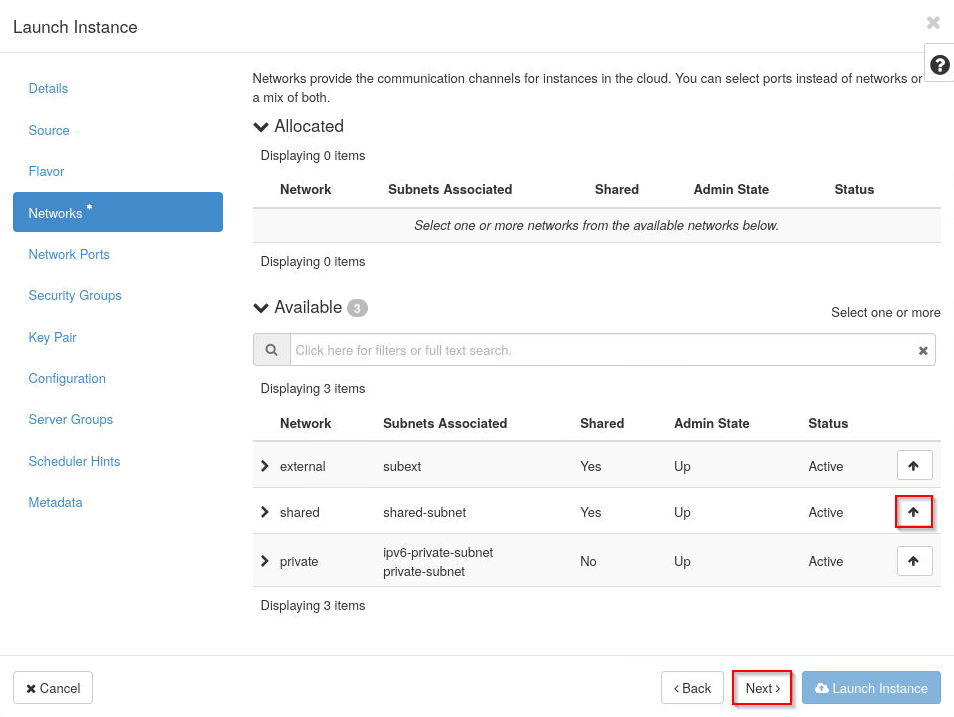
\includegraphics[width=\linewidth]{images/part1/step22.png}
    \end{center}

    \begin{stopbox}{}
        Before proceeding to the next step, confirm that \textbf{shared} appears underneath the \textit{Allocated}
        section.
    \end{stopbox}

    \item In the \textit{Network Ports} tab, click \textbf{Next}.
    
    \begin{center}
        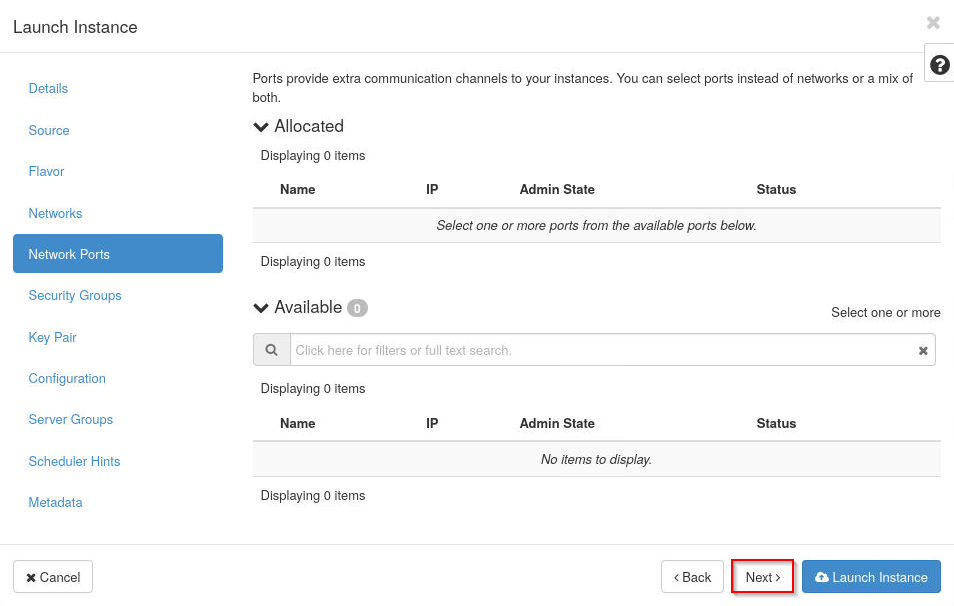
\includegraphics[width=\linewidth]{images/part1/step23.png}
    \end{center}

    \item In the \textit{Security Groups} tab, click the $\downarrow$ symbol in the same row as \textbf{default}, and
    click the $\uparrow$ symbol in the same row as \textbf{dev-secgroup}. Click \textbf{Next}.

    \begin{center}
        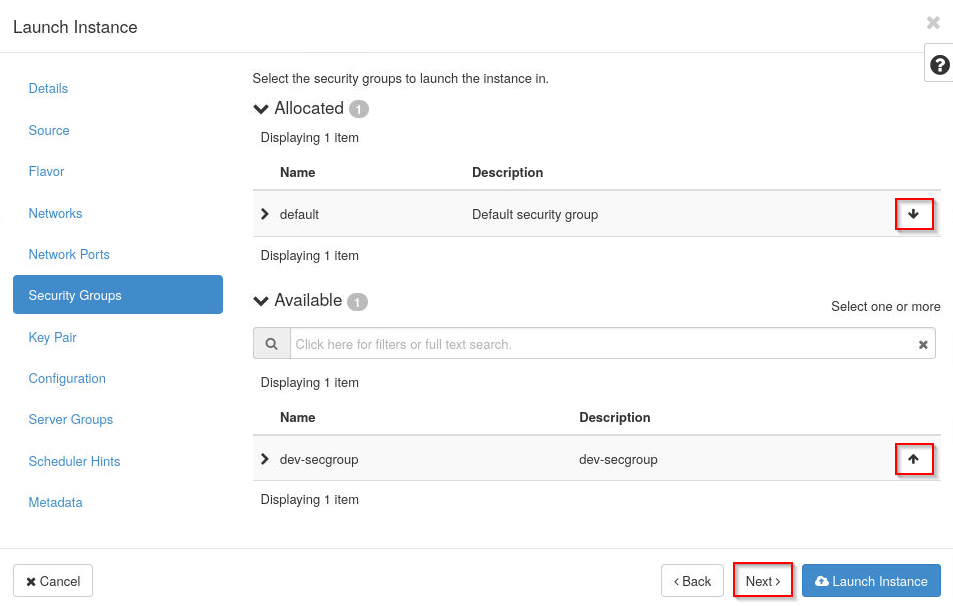
\includegraphics[width=\linewidth]{images/part1/step24.png}
    \end{center}

    \begin{stopbox}{}
        Before proceeding to the next step, confirm that only \textbf{dev-secgroup} appears underneath the
        \textit{Allocated} section.
    \end{stopbox}

    \item In the \textit{Key Pair} tab, ensure that the key pair \textbf{dev-keypair} has been selected and is
    underneath the \textit{Allocated} section. Click \textbf{Next}.

    \begin{center}
        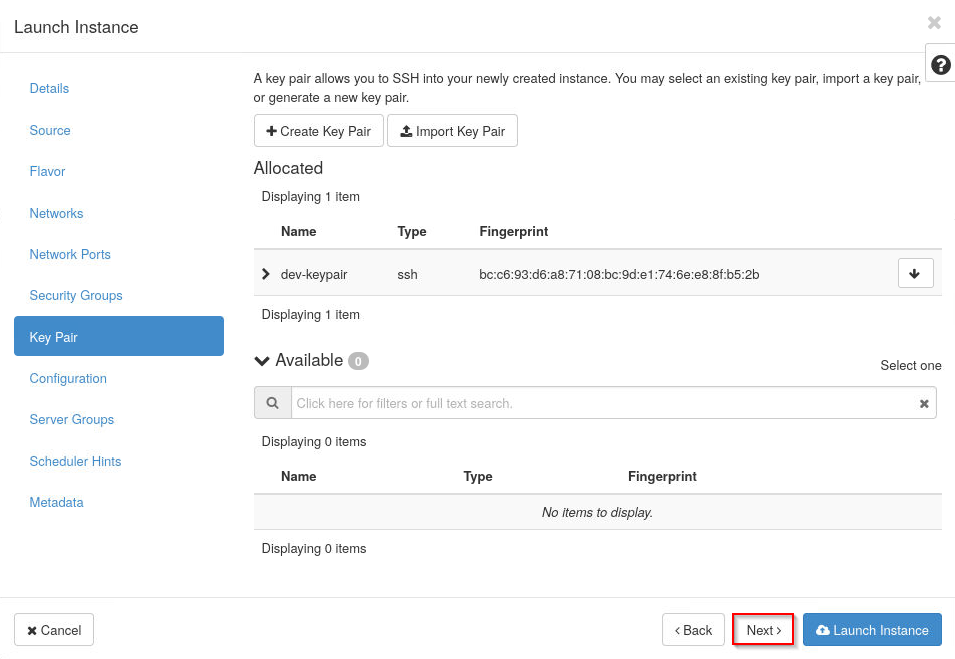
\includegraphics[width=\linewidth]{images/part1/step25.png}
    \end{center}

    \item In the \textit{Configuration} tab, populate the \textbf{Customization Script} field with the content below.
    Once finished, click \textbf{Launch Instance}.
\begin{lstlisting}
#!/bin/bash
echo 'Hello, world!' > /root/hello.txt
\end{lstlisting}

    \begin{center}
        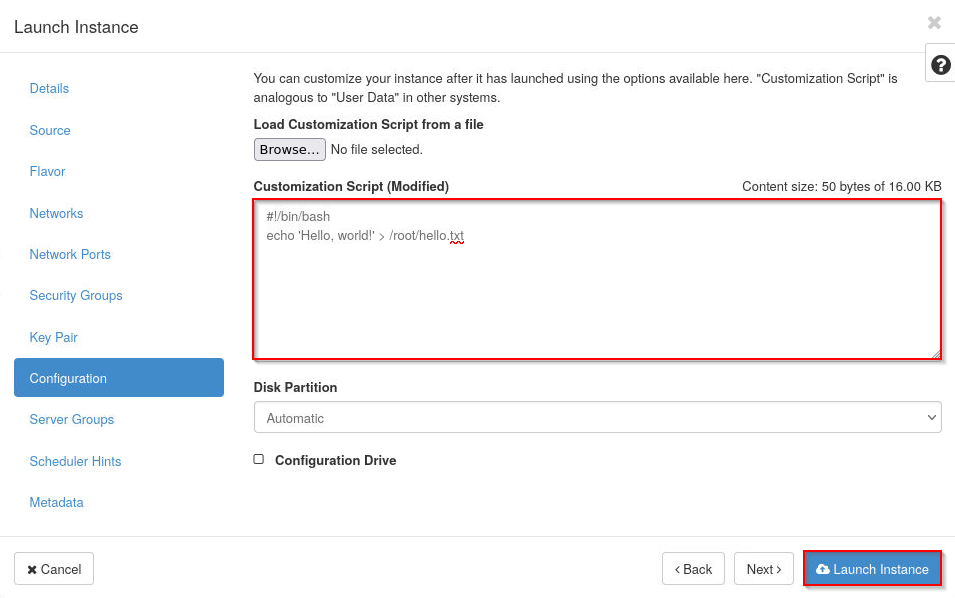
\includegraphics[width=\linewidth]{images/part1/step26.png}
    \end{center}

    \begin{tipbox}{}
        A customization script can be used to perform many commands automatically upon instance creation, such as
        installing packages, configuring a host name, etc. The simple script above is just an example.
    \end{tipbox}

    \item Once the status for \textbf{instance1} is \textbf{Active}, attach a floating IP address to it. Select
    \textbf{Associate Floating IP} from the dropdown menu next to \textbf{Create Snapshot} in the row for the instance.

    \begin{center}
        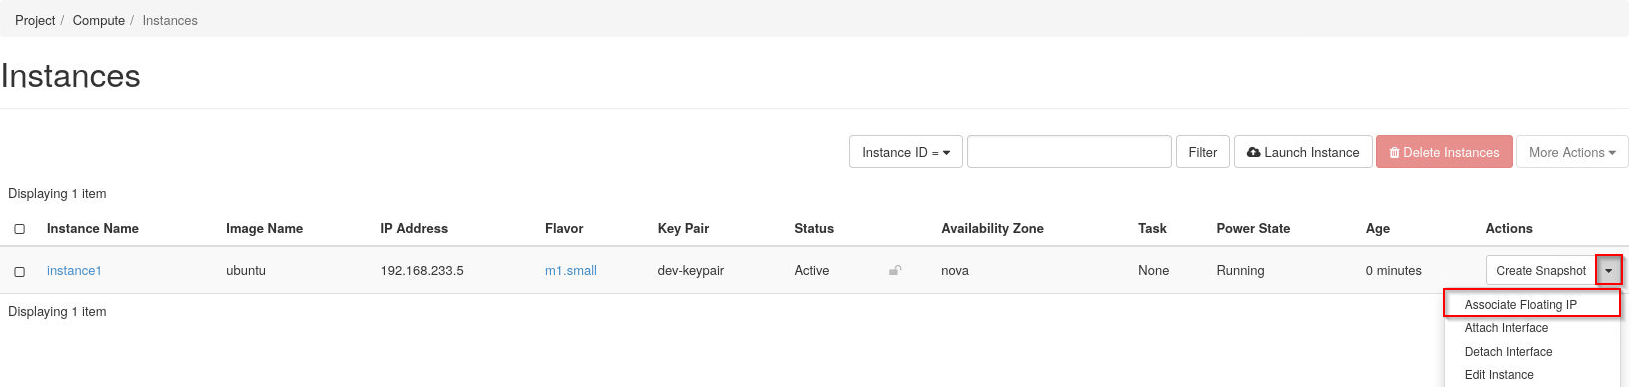
\includegraphics[width=\linewidth]{images/part1/step27.png}
    \end{center}

    \item Select any one of the IP addresses from the \textit{IP Address} dropdown and select
    \textbf{instance1: 192.168.233.XYZ} as the \textit{Port to be associated}. Click \textbf{Associate}.

    \begin{center}
        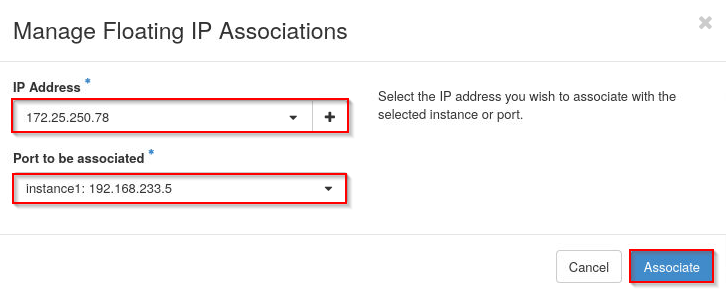
\includegraphics[width=\linewidth]{images/part1/step28.png}
    \end{center}

    \item To verify that the customization script worked, first click on \textbf{instance1} under the
    \textit{Instance Name} column, then navigate to the \textit{Console} tab if you are not directed there
    automatically. Log into the instance as \textbf{root} with the password \textbf{secret}.

    \begin{center}
        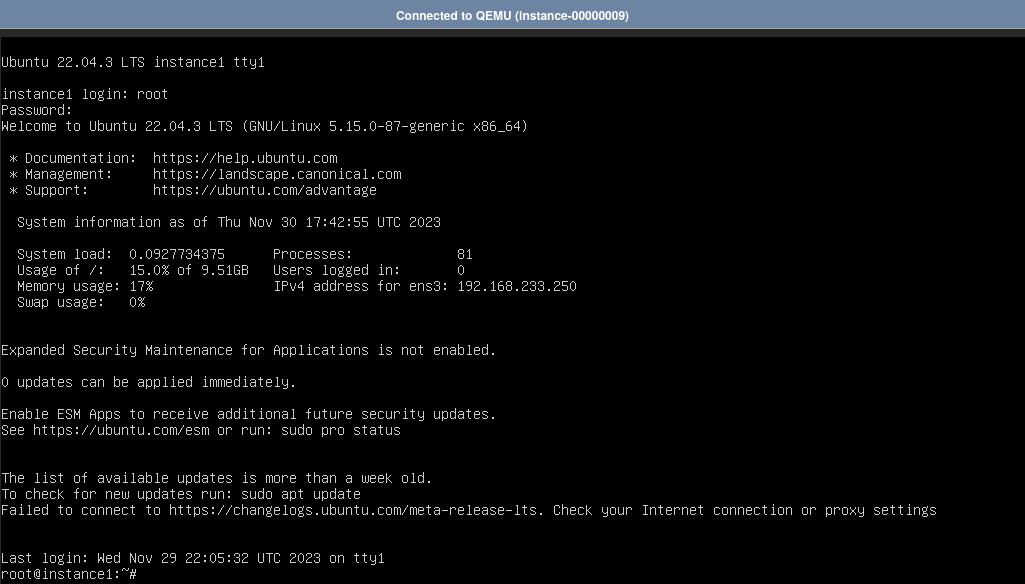
\includegraphics[width=\linewidth]{images/part1/step29.png}
    \end{center}

    \item Check \textbf{/var/log/cloud-init.log} to confirm that \textbf{cloud-init} ran. Use the \textbf{\texttt{tail}}
    command to print the last 10 lines of the log.
\begin{lstlisting}
root@instance1:~# tail /var/log/cloud-init.log
\end{lstlisting}

    \begin{center}
        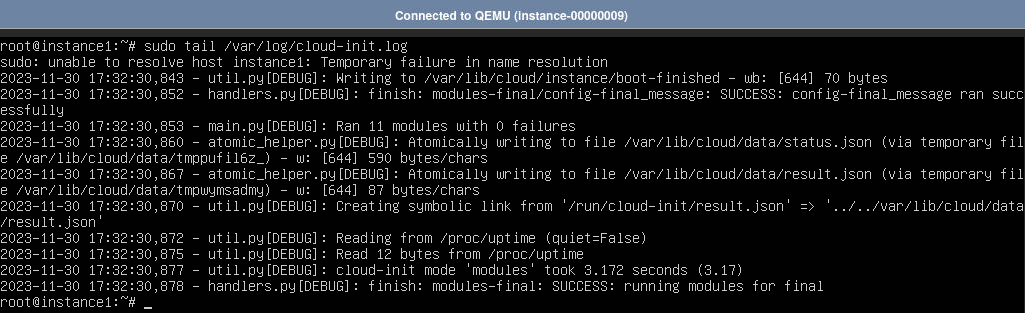
\includegraphics[width=\linewidth]{images/part1/step30.png}
    \end{center}

    \item Ensure that the \textbf{/root/hello.txt} file exists and has the correct content.
\begin{lstlisting}
root@instance1:~# cat /root/hello.txt
\end{lstlisting}

    \begin{center}
        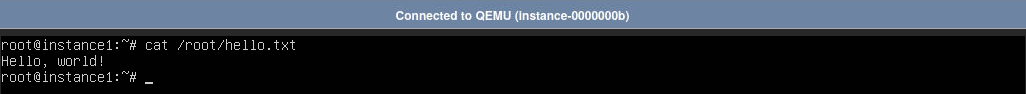
\includegraphics[width=\linewidth]{images/part1/step31.png}
    \end{center}

    \item Log out of the \textit{Horizon Dashboard} and close the web browser.

    \item Focus back on the terminal and delete \textbf{instance1}.
\begin{lstlisting}
ubuntu@workstation:~$ openstack server delete instance1
\end{lstlisting}

    \begin{center}
        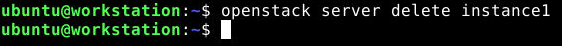
\includegraphics[width=\linewidth]{images/part1/step33.png}
    \end{center}

    \item Another instance will be created and customized using the \textit{OpenStack Unified CLI}. First, create a
    \textbf{user-data} script that will be attached to the instance at creation. Create a script called
    \textbf{\texttildemid/hello} that matches the content shown below. Press \textbf{CTRL+X}, then \textbf{Y} to
    accept the file changes. Press \textbf{Enter} to confirm and exit back to the terminal.
\begin{lstlisting}
ubuntu@workstation: nano ~/hello
\end{lstlisting}
\begin{lstlisting}
    #!/bin/bash
    echo 'Hello, world!' > /root/hello.txt
\end{lstlisting}

    \begin{center}
        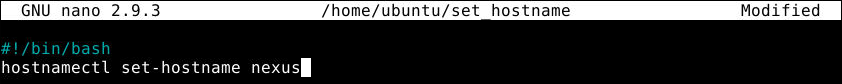
\includegraphics[width=\linewidth]{images/part1/step34.png}
    \end{center}

    \item Launch an instance using the \textbf{user-data} option with the previously created script to perform the
    customization. Use the \textbf{ubuntu} image, the \textbf{m1.small} flavor, the \textbf{shared} network, the
    \textbf{dev-secgroup} security group, and the \textbf{dev-keypair} key pair.
\begin{lstlisting}
ubuntu@workstation: openstack server create \
> --image ubuntu \
> --flavor m1.small \
> --nic net-id=shared \
> --security-group dev-secgroup \
> --key-name dev-keypair \
> --user-data ~/hello \
> --wait instance2
\end{lstlisting}

    \begin{center}
        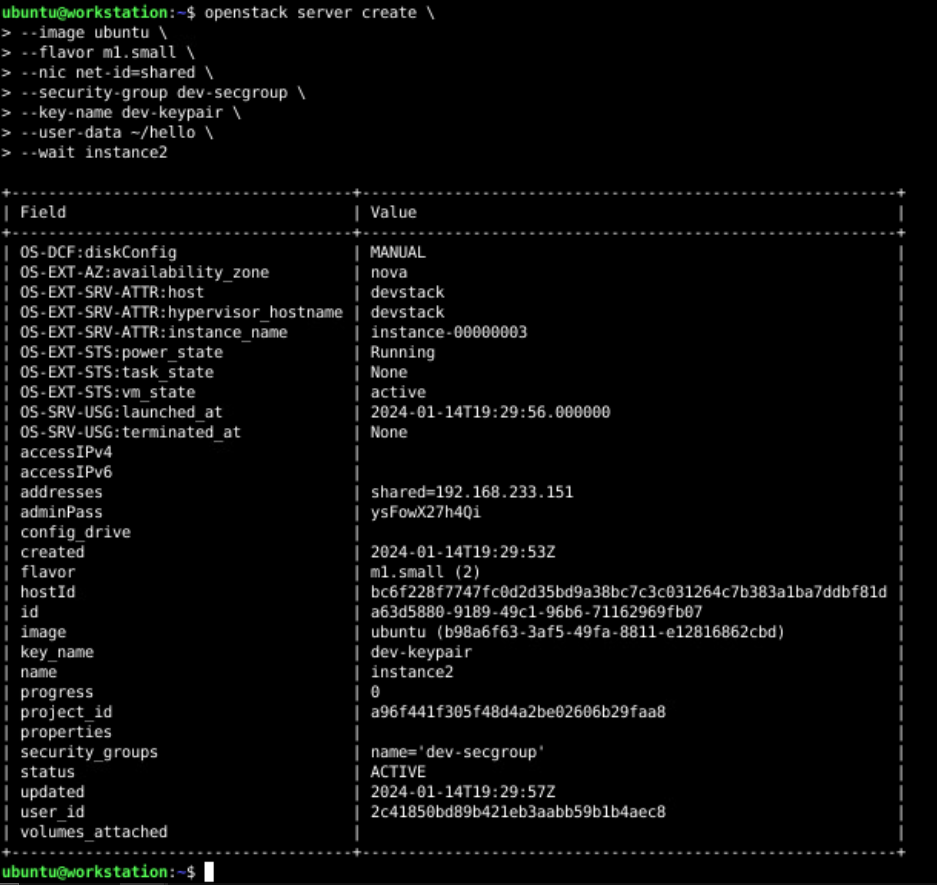
\includegraphics[width=\linewidth]{images/part1/step35.png}
    \end{center}

    \item Verify that the status of the \textbf{instance2} instance is \textbf{ACTIVE}.
\begin{lstlisting}
ubuntu@workstation: openstack server list
\end{lstlisting}

    \begin{center}
        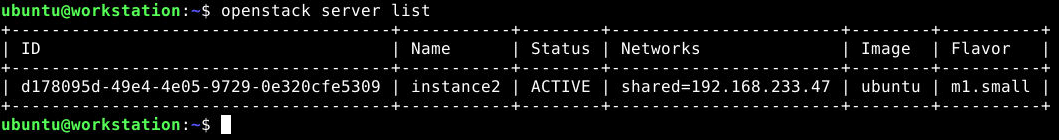
\includegraphics[width=\linewidth]{images/part1/step36.png}
    \end{center}

    \item Generate another floating IP address to assign to this instance. Take note of the IP address generated, which
    is listed in the \textit{name} row in the output from the below command.
\begin{lstlisting}
ubuntu@workstation:~$ openstack floating ip create external
\end{lstlisting}

    \begin{center}
        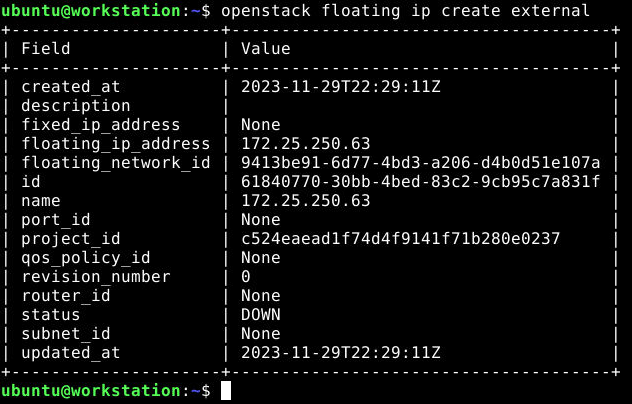
\includegraphics[width=\linewidth]{images/part1/step37.png}
    \end{center}

    \item Assign the floating IP generated from the last step to \textbf{instance2}.
\begin{lstlisting}
ubuntu@workstation:~$ openstack server add floating ip \
instance2 172.25.250.63
\end{lstlisting}

    \begin{center}
        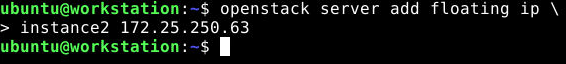
\includegraphics[width=\linewidth]{images/part1/step38.png}
    \end{center}

    \begin{notebox}{}
        The actual value of your floating IP address may be different.
    \end{notebox}

\end{enumerate}

\section{Verify Customized Instances}
\label{sec:verify_customized_instances}
In this task, you will verify that \textbf{\texttt{cloud-init}} has correctly customized the two instances created in the
previous section.

\begin{enumerate}
    \item If a terminal window is not already open, open one and source the admin credentials from the 
    \textbf{\texttildemid/keystonerc-admin} file.

    \item Determine the floating IP address associated with \textbf{instance2}. Remember that the floating IP address is
    in the \textbf{172.25.250.0/24} subnet.
\begin{lstlisting}
ubuntu@workstation: openstack server show instance2 \
> | grep address
\end{lstlisting}

    \begin{center}
        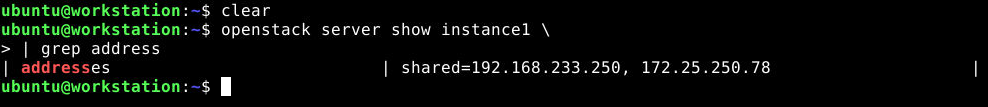
\includegraphics[width=\linewidth]{images/part2/step2.png}
    \end{center}

    \begin{notebox}{}
        The floating IP addresses in your output may differ from these examples.
    \end{notebox}

    \item Use the \textbf{\texttt{scp}} command to copy the \textbf{\texttildemid/Downloads/dev-keypair.pem} file to
    the \textbf{devstack} machine. You will be prompted to enter the password for \textbf{ubuntu@192.168.1.20}. The
    password can be found on the EZSetup page for the lab by clicking on the \textbf{devstack} machine, then 
\begin{lstlisting}
ubuntu@workstation:~$ scp ~/Downloads/dev-keypair.pem \
> ubuntu@192.168.1.20:~/dev-keypair.pem
\end{lstlisting}

    \begin{center}
        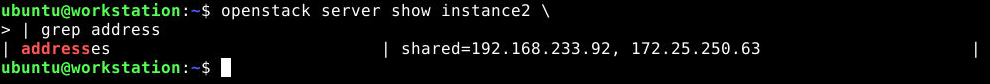
\includegraphics[width=\linewidth]{images/part2/step3.png}
    \end{center}

    \item SSH into the \textbf{devstack} machine. The password is the same as the last step.
\begin{lstlisting}
ubuntu@workstation:~$ ssh 192.168.1.20
\end{lstlisting}

    \begin{center}
        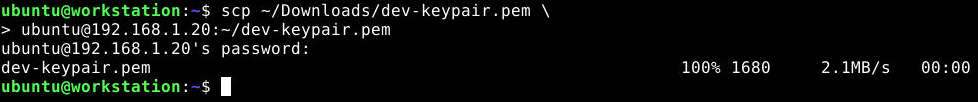
\includegraphics[width=\linewidth]{images/part2/step4.png}
    \end{center}

    \item SSH into \textbf{instance2} using the \textbf{dev-keypair} private key.
\begin{lstlisting}
ubuntu@devstack:~$ ssh -i ~/dev-keypair.pem 172.25.250.63
\end{lstlisting}

    \begin{center}
        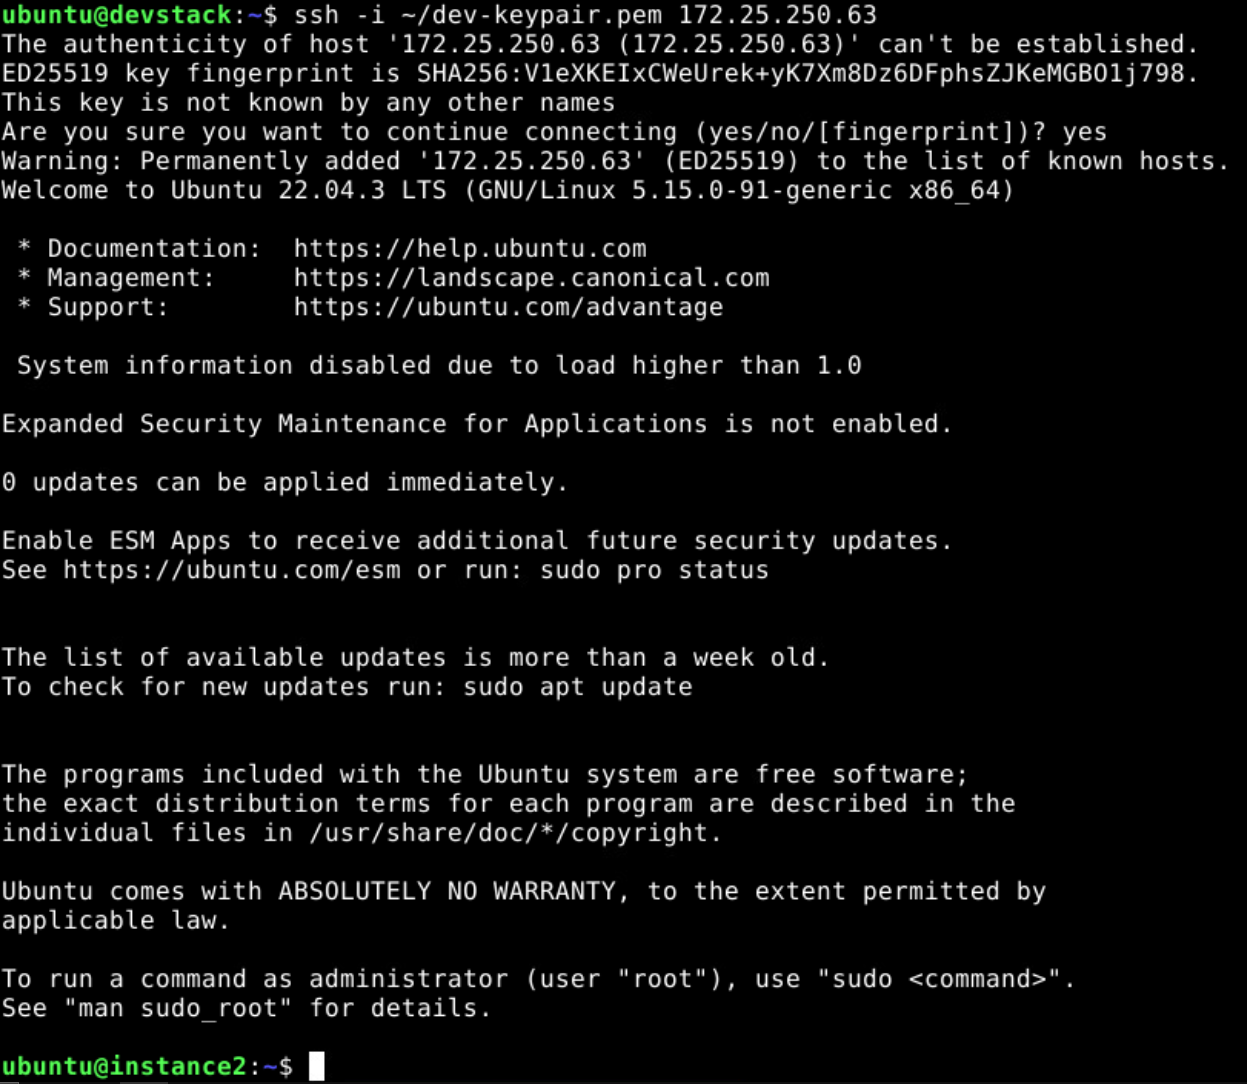
\includegraphics[width=\linewidth]{images/part2/step5.png}
    \end{center}

    \begin{notebox}{}
        It may take several minutes for the instance to fully boot and be available for an SSH connection.
    \end{notebox}

    \item Check \textbf{/var/log/cloud-init.log} to confirm that the \textbf{cloud-init} script ran.
\begin{lstlisting}
ubuntu@instance2:~$ sudo tail /var/log/cloud-init.log
\end{lstlisting}

    \begin{center}
        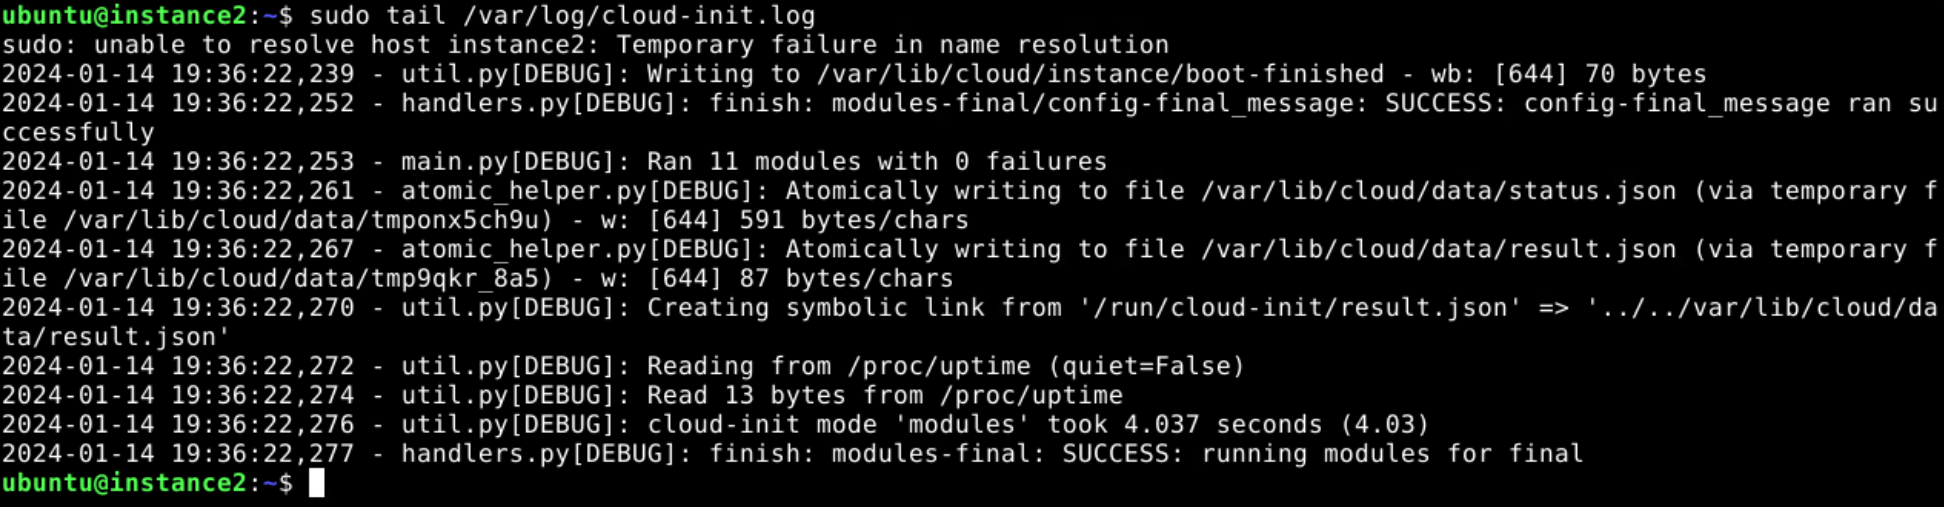
\includegraphics[width=\linewidth]{images/part2/step6.png}
    \end{center}

    \item Ensure that the \textbf{/root/hello.txt} file exists and has the correct content.
\begin{lstlisting}
ubuntu@instance2:~# cat /root/hello.txt
\end{lstlisting}

    \begin{center}
        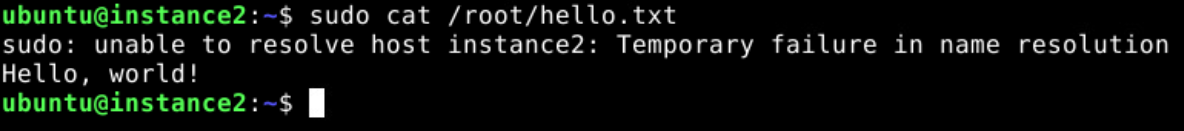
\includegraphics[width=\linewidth]{images/part2/step7.png}
    \end{center}

    \item The lab is now complete.

\end{enumerate}

\end{document}
